% Impostazioni principali
\documentclass[t, compress, mathserif]{beamer}



%         ----------------------------------------------         %
%        /                                              \        %
%--------               START PREAMBLE                   --------%
%        \                                              /        %
%         ----------------------------------------------         %

% Titolo che appare nella prima slide del documento
\newcommand{\titolo}{Basic Mathematics}
\newcommand{\sottotitolo}{}

% Titolo che appare nella barra in basso di ogni slide, al centro
% Sono due variabili:
% * una puo' essere utilizzata per l'intero corso. Se impostata nel preambolo sovrascrive quella di seguito.
% * l'altra puo' identificare ciascun documento
\newcommand{\titolocompleto}{Quantitative Methods for Business - }
\newcommand{\titoloshort}{\titolo}

% Numero di capitolo o altro nome che appare in basso di ogni slide, vicino al numero di pagina
\newcommand{\numerocapitolo}{Chapter 1}

% Include il documento che contiene il preambolo

%%%%%%%%%%%%%%%%%%%%%%%%%%%%%%%%%%%%%%%%%%%%%%%%%%%%%%%%%%%%%%%%%%%%%%%%%%%%%%
%%%%%%%%%%%%%%%%%%%%%%%%%%%% VARIABILI DA DEFINIRE %%%%%%%%%%%%%%%%%%%%%%%%%%%
%%%%%%%%%%%%%%%%%%%%%%%%%%%%%%%%%%%%%%%%%%%%%%%%%%%%%%%%%%%%%%%%%%%%%%%%%%%%%%

% Titolo che appare nella barra in basso di ogni slide, al centro
% Se impostato ha la precedenza rispetto a quello di ogni singola slide

%\renewcommand{\titolocompleto}{}

% non c'e' newcommand{\sottotitolo} perche' viene definito in ogni slide
\newcommand{\data}{}



%%%%%%%%%%%%%%%%%%%%%%%%%%%%%%%%%%%%%%%%%%%%%%%%%%%%%%%%%%%%%%%%%%%%%%%%%%%%%%
%%%%%%%%%%%%%%%%%%%%%%%%%%%%%%%%%% PACKAGES %%%%%%%%%%%%%%%%%%%%%%%%%%%%%%%%%%
%%%%%%%%%%%%%%%%%%%%%%%%%%%%%%%%%%%%%%%%%%%%%%%%%%%%%%%%%%%%%%%%%%%%%%%%%%%%%%
\usepackage[latin1]{inputenc}   
\usepackage{graphicx}
\usepackage{rotating}
\usepackage{rotfloat}
\usepackage{color}
\usepackage{colortbl}
\usepackage{../includeTex/floatflt}
\usepackage{tikz}
\usepackage{hyperref}
\usepackage{pgfpages} 
\usepackage{ifthen}
\usepackage{wasysym}
\usepackage{multirow}



%%%%%%%%%%%%%%%%%%%%%%%%%%%%%%%%%%%%%%%%%%%%%%%%%%%%%%%%%%%%%%%%%%%%%%%%%%%%%%
%%%%%%%%%%%%%%%%%%%%%%%%%%%% IMPOSTAZIONI GENERALI %%%%%%%%%%%%%%%%%%%%%%%%%%%
%%%%%%%%%%%%%%%%%%%%%%%%%%%%%%%%%%%%%%%%%%%%%%%%%%%%%%%%%%%%%%%%%%%%%%%%%%%%%%

% Beamer theme
%\usetheme{CambridgeUS}      
\usetheme{Madrid}      

% Immagini da visualizzare
\newcommand{\materiale}{minitab}

% Path delle immagini
\graphicspath{{../images/}}

% Per caricare le formule matematiche con il giusto font 
% Questo sostituisce l'opzione mathserif di documentclass (obsoleta) 
\usefonttheme[onlymath]{serif}      

     

%%%%%%%%%%%%%%%%%%%%%%%%%%%%%%%%%%%%%%%%%%%%%%%%%%%%%%%%%%%%%%%%%%%%%%%%%%%%%%
%%%%%%%%%%%%%%%%%%%%%%%%%%%%%%%%%%% COLORI %%%%%%%%%%%%%%%%%%%%%%%%%%%%%%%%%%%
%%%%%%%%%%%%%%%%%%%%%%%%%%%%%%%%%%%%%%%%%%%%%%%%%%%%%%%%%%%%%%%%%%%%%%%%%%%%%%

\definecolor{grigio}{rgb}{0.46,0.48,0.48}
\definecolor{giallo}{rgb}{1,0.84,0}
\definecolor{coolred}{rgb}{0.83,0.06,0.27}
\definecolor{arancio}{rgb}{0.97,0.46,0.09}
\definecolor{verde}{rgb}{0.25,0.78,0.25}
\definecolor{qblu}{rgb}{0.24,0.27,0.74}
\definecolor{azzurro}{rgb}{0.37,0.91,0.90}

\definecolor{grigio}{rgb}{0.46,0.48,0.48}
\definecolor{blu}{rgb}{0.25,0.28,0.78}

\definecolor{sfondoScopo}{rgb}{0.75,0.785,0.83}
\definecolor{darkred}{named}{qblu}
\definecolor{blue}{named}{qblu}

\setbeamercolor{scopo}{bg=sfondoScopo}
\setbeamercolor{section in toc}{fg=black,bg=white}
\setbeamercolor{alerted text}{fg=darkred!80!gray}
\setbeamercolor{palette primary}{fg=darkred!60!black,bg=gray!30!white}
\setbeamercolor{palette secondary}{fg=darkred!70!black,bg=gray!15!white}
\setbeamercolor{palette tertiary}{bg=darkred!80!black,fg=gray!10!white}
\setbeamercolor{palette quaternary}{fg=darkred,bg=gray!5!white}

\setbeamercolor{sidebar}{fg=darkred,bg=gray!15!white}
\setbeamercolor{palette sidebar primary}{fg=darkred!10!black}
\setbeamercolor{palette sidebar secondary}{fg=white}
\setbeamercolor{palette sidebar tertiary}{fg=darkred!50!black}
\setbeamercolor{palette sidebar quaternary}{fg=gray!10!white}

\setbeamercolor{titlelike}{parent=pallette primary,fg=darkred}
\setbeamercolor{frametitle}{bg=gray!10!white}
\setbeamercolor{frametitle right}{bg=gray!60!white}

\setbeamercolor{separation line}{}
\setbeamercolor{fine separation line}{}

%% Definizione dei colori da assegnare ai box
\setbeamercolor{postit}{fg=white,bg=qblu}
\setbeamercolor{postut}{fg=qblu,bg=gray!60!white}

%% Definizione dei colori per i diagrammi
\definecolor{bloccoIniziale}{rgb}{0.94,0.93,0.48}
\definecolor{bloccoFinale}{rgb}{0.86,0.25,0.27}
\definecolor{blocco}{rgb}{0.56,0.58,0.77}
\definecolor{bloccoSospeso}{rgb}{0.94,0.81,0.36}



%%%%%%%%%%%%%%%%%%%%%%%%%%%%%%%%%%%%%%%%%%%%%%%%%%%%%%%%%%%%%%%%%%%%%%%%%%%%%%
%%%%%%%%%%%%%%%%%%%%%%%%% STRUTTURA DELLE DIAPOSITIVE %%%%%%%%%%%%%%%%%%%%%%%%
%%%%%%%%%%%%%%%%%%%%%%%%%%%%%%%%%%%%%%%%%%%%%%%%%%%%%%%%%%%%%%%%%%%%%%%%%%%%%%

% Intestazione
\setbeamertemplate{headline}
{
  \leavevmode%
  \hbox{%
  \begin{beamercolorbox}[wd=.5\paperwidth,ht=2.25ex,dp=1ex,right]{section in head/foot}%
    \usebeamerfont{section in head/foot}\insertsectionhead\hspace*{2ex}
  \end{beamercolorbox}%
  \begin{beamercolorbox}[wd=.5\paperwidth,ht=2.25ex,dp=1ex,left]{subsection in head/foot}%
    \usebeamerfont{subsection in head/foot}\hspace*{2ex}\insertsubsectionhead
  \end{beamercolorbox}}%
  \vskip0pt%
}

% Pie' di pagina
\setbeamertemplate{footline}
{
  \hbox{%
    \begin{beamercolorbox}[wd=.20\paperwidth, ht = 2.25ex, dp = 1ex, center]{palette sidebar secondary}%
      \usebeamerfont{author in head/foot}%\insertshortauthor~~(\insertshortinstitute) 
      
\includegraphics[width=1.5cm]{QUANTIDE.jpg}
    \end{beamercolorbox}%
    \begin{beamercolorbox}[wd=.57\paperwidth, ht = 2.25ex, dp = 1ex, center]{title in head/foot}%
      \usebeamerfont{title in head/foot}{\titolocompleto \titoloshort}
    \end{beamercolorbox}%
    \begin{beamercolorbox}[wd=.13\paperwidth, ht = 2.25ex, dp = 1ex, left]{date in head/foot}%
      \hspace*{0.4em} \usebeamerfont{date in head/foot} {\numerocapitolo}
    \end{beamercolorbox}%
    \begin{beamercolorbox}[wd=.10\paperwidth, ht = 2.25ex, dp = 1ex, right]{date in head/foot}%
       \usebeamerfont{date in head/foot} \insertframenumber{} / \inserttotalframenumber \hspace*{2ex} 
    \end{beamercolorbox}%
  }%
  \vskip0pt%
}



%%%%%%%%%%%%%%%%%%%%%%%%%%%%%%%%%%%%%%%%%%%%%%%%%%%%%%%%%%%%%%%%%%%%%%%%%%%%%%
%%%%%%%%%%%%%%%%%%%%%%%%%%% STILE DELLE DIAPOSITIVE %%%%%%%%%%%%%%%%%%%%%%%%%%
%%%%%%%%%%%%%%%%%%%%%%%%%%%%%%%%%%%%%%%%%%%%%%%%%%%%%%%%%%%%%%%%%%%%%%%%%%%%%%

% Simboli di navigazione
\setbeamertemplate{navigation symbols}{}

% Modifica lo stile dell'elenco (di primo livello)
\useitemizeitemtemplate{$\star$} % Usa la stella

% Interlinea (fattore di scala; NON e' un valore assoluto)
\renewcommand{\baselinestretch}{1.2}  

% Definisci stile per vettori e matrici
\newcommand{\vect}[1]{\boldsymbol{\underline{#1}}} % Grassetto e sottolineato
\newcommand{\matr}[1]{\boldsymbol{#1}} % Grassetto

% Definire stile per valore assoluto
\providecommand{\abs}[1]{\lvert#1\rvert}
\providecommand{\norm}[1]{\lVert#1\rVert}

% Cambiare il nome delle figure e delle tabelle
\renewcommand{\figurename}{Figura}
\renewcommand{\tablename}{Tabella}

% Definizione sezioni, ecc.
\newcommand{\livelloA}{\section}
\newcommand{\livelloB}{\subsection}
\newcommand{\livelloC}{\subsubsection}

% Livello di profondita' del 'content panel' del PDF
% \hypersetup{bookmarksdepth=4} % il valore di default va bene

% Definizione prima slide
\title{\textbf{\titolo}}
\author{\sottotitolo}
\date{\data}






%         ----------------------------------------------         %
%        /                                              \        %
%--------               START DOCUMENT                   --------%
%        \                                              /        %
%         ----------------------------------------------         %

\begin{document}

% Pagina del titolo
\frame{\titlepage}

% Indice
% \begin{frame}
% 	 \tableofcontents
% \end{frame}

% Documento
% I soli contenuti del documento sono in un file esterno. Questo semplifica enormemente le cose qualora si volessero creare dei manuali (singoli documenti) a partire da diversi documenti.
\livelloA{Numbers and Symbols}
\livelloB{Basic Mathematics}
\begin{frame}
  \begin{itemize}
  	\item Add, subtract, multiply and divide numbers
  	\item Combine operations and use brackets
  	\item Rounding to decimal places or significant figures
  	\item scientific notation
  	\item Use symbols to represent relationships
  	\item constants and variables
  	\item Evaluate expressions
  	\item Understand the concept of a model
  	\item Use a spreadsheet
  	\item Simplify expressions containing symbols
  \end{itemize}
\end{frame}
%%%%%%%%%%%%%%%%%%%%%%%%%%%%%%%%%%%%%%%%%
\livelloA{What do I need to know?}
\livelloB{Basic Mathematics}
\begin{frame}
We assume  that:
\begin{itemize}

	\item you know how to add, subtract, multiply and divide positive numbers
	\item you can cope with numbers like 5.123 in which the fractional part is given using decimal places
\end{itemize}
\end{frame}
%%%%%%%%%%%%%%%%%%%%%%%%%%%%%%%%%%%%%%%%%%%%%
\livelloA{Positive and negative Numbers}
\livelloB{Basic Mathematics}
\begin{frame}
\begin{itemize}
\item ... -6  -5  -4  -3  -2  -1   0   1   2   3   4   5   6...
\item 0
\item 2, 4, 5
\item 2.14, 3.76, 21.9351
\item -2, -4, -5
\item -2.43, -12.54, -17.9136
\end{itemize}
\end{frame}
%%%%%%%%%%%%%%%%%%%%%%%%%%%%%%%%%%%%%%%%%
\livelloA{Adding and Subtracting}
\livelloB{Basic Mathematics}
\begin{frame}
\begin{itemize}
\item OPPOSITE SIGNS
\begin{itemize}
\item + (- number) or - (+ number) gives a -
\item 3 + (-5) = 3 - 5  = -2
\end{itemize}
\item SAME SIGNS
\begin{itemize}
\item - (- number) or + (+ number) gives a +
\item (-3) - 7 = -10
\item 12.42 - (-3.1) = 12.42 + 3.1 = 15.52
\end{itemize}
\end{itemize}
\end{frame}
%%%%%%%%%%%%%%%%%%%%%%%%%%%%%%%%%%%%%%%%%
\livelloA{Multiplying Numbers}
\livelloB{Basic Mathematics}
\begin{frame}
\begin{itemize}

	\item the same signs gives a $+$
	\item different signs gives a $-$
	  \vspace*{.35cm}
	\item + x + = +   2 x 3 = 6
	\item + x - = +   2 x (-3) = -6
	\item - x + = -   (-2) x 3 = -6
	\item - x - = +   (-2) x (-3) = -6
\end{itemize}
\end{frame}
%%%%%%%%%%%%%%%%%%%%%%%%%%%%%%%%%%%%%%%%%
\livelloA{Dividing Numbers}
\livelloB{Basic Mathematics}
\begin{frame}
\begin{itemize}

	\item the same signs gives a $+$
	\item different signs gives a $-$
	  \vspace*{.35cm}
	\item $+ \div  + = +$   $6 \div 3 = 2$
	\item $+ \div  - = -$   $(-6) \div 3 = -2$
	\item $- \div  + = -$   $6 \div (-3) = -2$
	\item $- \div  - = +$   $(-6) \div (-3) = 2$
\end{itemize}
\end{frame}
%%%%%%%%%%%%%%%%%%%%%%%%%%%%%%%%%%%%%%%%%
\livelloA{Combining Operations}
\livelloB{Basic Mathematics}
\begin{frame}
In order:
\begin{itemize}
	\item Brackets
	\item Multiply and Divide (from left to right)
	\item Add and Subtract (from left to right)
	\vspace*{.35cm}
	\item $2 \times 2 \times  (27 \div 3) + (1 - 20)$
	\item $= 2 \times 2 \times (9) + (-19)$
	\item $= 36 - 20$
	\item $= 17$
\end{itemize}
\end{frame}
%%%%%%%%%%%%%%%%%%%%%%%%%%%%%%%%%%%%%%%%%
\livelloA{Rounding}
\livelloB{Basic Mathematics}
\begin{frame}

\begin{itemize}
\item To decimal places $-$ the number of digits after a decimal point
\item 1234.56789
\vspace*{.35cm}
\begin{itemize}
	\item is $1234.568$ to $3$ decimal places
	\item is $1234.6$ to $1$ decimal place
\end{itemize}
\end{itemize}
\end{frame}
%%%%%%%%%%%%%%%%%%%%%%%%%%%%%%%%%%%%%%%%%
\livelloA{Scientific Notation}
\livelloB{Basic Mathematics}
\begin{frame}
\begin{itemize}
	\item $a \times 10^b$
	\begin{itemize}
		\item Where $1 \le a < 10$
		\item $B$ is an integer
	\end{itemize}
	\vspace*{.35cm}
		\item $12000 = 1.2 \times 10^4$
		\item $0.0012 = 1.2 \times 10^{-3}$
	\end{itemize}
\end{frame}
%%%%%%%%%%%%%%%%%%%%%%%%%%%%%%%%%%%%%%%%%
\livelloA{Letters and Symbols}
\livelloB{Basic Mathematics}
\begin{frame}
\begin{itemize}
	\item Letters are used to give a general representation of a constant or variable
	\vspace*{.35cm}
	\item $S =$ the speed of a car:  variable
	\item W = the weight of a book - constant
	\end{itemize}
\end{frame}
%%%%%%%%%%%%%%%%%%%%%%%%%%%%%%%%%%%%%%%%%
\livelloA{Letters are brought together in equations to show relationships}
\livelloB{Basic Mathematics}
\begin{frame}
\begin{itemize}
		\item $C =$ the cost of hiring a boat for a trip
		\item $F =$ the fixed costs of the hire
		\item $P =$ the cost of petrol an hour (variable)
		\item $H =$ the time spent on a trip (variable)
		\item $C = F + HP$
		\vspace*{.35cm}
		\item If n people hire the boat each pays:
		\item $\frac{C}{n} = \frac{F + NP}{n}$
		\end{itemize}
\end{frame}
%%%%%%%%%%%%%%%%%%%%%%%%%%%%%%%%%%%%%%%%%
\livelloA{Model}
\livelloB{Basic Mathematics}
\begin{frame}
\begin{itemize}
	\item The relationships form models of problems
	\item Finding a solution to a problem means solving the equations
	\item We have to find previously unknown from the known ones
	\item For this we have to manipulate the equations into the required form
\end{itemize}
\end{frame}
%%%%%%%%%%%%%%%%%%%%%%%%%%%%%%%%%%%%%%%%%
\livelloA{Working With Symbols}
\livelloB{Basic Mathematics}
\begin{frame}
\begin{itemize}
	\item The rules for addition, subtraction, multiplication and division are exactly the same as for arithmetic with numbers
	\begin{itemize}
		\item $-(-a) = a \; -(+a) = -a \; etc ...$
		\item $a \times(-b) = -ab \; (-a) \times (-b) = ab \; etc ...$
		\item $ \frac{a}{-b} = \frac{-a}{b} \; \frac{-a}{-b} \frac{a}{b} \; etc ...$
		\vspace*{.35cm}
		\item Remember explicit multiplication $2a = 2 \times a$
	\end{itemize}
	\end{itemize}
\end{frame}
%%%%%%%%%%%%%%%%%%%%%%%%%%%%%%%%%%%%%%%%%
\livelloA{Collecting Terms Together}
\livelloB{Basic Mathematics}
\begin{frame}
\begin{itemize}
	\item Often we have to collect like terms together
	\begin{itemize}
		\item $2pq + pq - 5pq  =  -2pq$
		\item $\frac{s}{2r} + \frac{4s}{2r}  =  \frac{5s}{2r}$
	\end{itemize}
	\end{itemize}
\end{frame}

%%%%%%%%%%%%%%%%%%%%%%%%%%%%%%%%%%%%%%%%%
\livelloA{Fractions}
\livelloB{Simplifying Expressions}

\begin{frame}
\begin{itemize}
	\item A fraction is:

	\item $ \frac{numerator}{denominator}$
	\item A fraction keeps the same value when you do the same thing to both the numerator and denominator.
	\item Dividing top and bottom means that
	\item $\frac{84}{162}  =  \frac{42}{81}  = \frac{14}{27}$
	\item When no further cancelling can be done, a fraction is in its simplest form.
	\end{itemize}
\end{frame}

%%%%%%%%%%%%%%%%%%%%%%%%%%%%%%%%%%%%%%%%%
\livelloA{Working whit fractions}
\livelloB{Simplifying Expressions}
\begin{frame}
Multiplying fractions
\begin{itemize}
	\item Multiply the numerators and the denominators
	\item $\frac{2}{3} \times \frac{4}{5}  =  \frac{8}{15}$
	\item $\frac{a}{b} \times \frac{c}{b} = \frac{ab}{cd}$
\end{itemize}
Dividing fractions
\begin{itemize}
	\item Turn the second fraction upside down and multiply
	\item $\frac{1}{2} \div \frac{2}{3}  =  \frac{1}{2} \times \frac{3}{2}  =  \frac{3}{4}$
	\item $\frac{a}{b} \div \frac{c}{d}  =  \frac{a}{b} \times \frac{d}{c}  =  \frac{ad}{bc}$
\end{itemize}
\end{frame}
%%%%%%%%%%%%%%%%%%%%%%%%%%%%%%%%%%%%%%%%%
\livelloA{Percentages}
\livelloB{Simplifying Expressions}
\begin{frame}
\begin{itemize}
	\item Percentages are the number of hundredths
	\item $ 5\% = 5 \div 100$
	\item $ 6\% of 300 = 300 \times \frac{6}{100}$
	\item $ \frac{25}{400} = \frac{6.25}{100} = 6.25\% $
\end{itemize}
\end{frame}

%%%%%%%%%%%%%%%%%%%%%%%%%%%%%%%%%%%%%%%%%
\livelloA{Brackets}
\livelloB{Simplifying Expressions}
\begin{frame}
Expanding Brackets
\begin{itemize}
	\item The value before a bracket is multiplied by everything inside the brackets
	\item $ a(b + c)  =  ab + ac$
	\item $ x(y + z) - xy  = xy+xz-xy  =  xz$
	\item $ \frac{b + c}{a}  = \frac{b}{c} + \frac{c}{a} $
\end{itemize}
Product of Brackets
\begin{itemize}
	\item Everything inside the first bracket is multiplied by everything inside the second bracket
	\item $(a + b)(c + d)  =  ac + ad + bc + bd$
	\item $ (x - 2)(y + 1)  =  xy - 2y + x - 2$
\end{itemize}
\end{frame}
%%%%%%%%%%%%%%%%%%%%%%%%%%%%%%%%%%%%%%%%%
\livelloA{Factorizing}
\livelloB{Simplifying Expressions}
\begin{frame}
The opposite of expanding brackets; means taking an equation and finding the factors
\begin{itemize}
	\item $ 5ma + 15 m  =  5m(a + 3)$
	\item $ y2+4y-5  =  (y + 5)(y - 1)$
	\item $ a^2 + 2ac + c2  =  (a + c)^2$
\end{itemize}
\end{frame}

%%%%%%%%%%%%%%%%%%%%%%%%%%%%%%%%%%%%%%%%%
\livelloA{Common Factors}
\livelloB{Simplifying Expressions}
\begin{frame}
Factorising is useful in solving equations
\begin{itemize}
	\item $ a^2 + 2ab +b^2  = (a + b)^2$
	\item $a^2 -2ab +b^2  =  (a - b)^2$
	\item $ a^2 - b^2  =  (a + b)(a - b)$
	\item $ a^2 + b^2  =  $
\end{itemize}
\end{frame}
%%%%%%%%%%%%%%%%%%%%%%%%%%%%%%%%%%%%%%%%%
\livelloA{Powers}
\livelloB{Simplifying Expressions}
\begin{frame}
Multiplying a value by itself a number of times
\begin{itemize}
	\item $a$ squared $= a \times a  =  a^2$
	\item $2$ cubed  $=  2 \times 2 \times 2  =  2^3  =  8$
	\item $-2$ to the power $4  =  (-2)^4  =  16$
	\item $ \frac{2}{3}$ to the power $5  =  (\frac{2}{3})^5  =  32/243$
	\item $a^0 = 1$ for any value of $a$

\end{itemize}
\end{frame}
%%%%%%%%%%%%%%%%%%%%%%%%%%%%%%%%%%%%%%%%%
\livelloA{Negative Powers}
\livelloB{Simplifying Expressions}
\begin{frame}
Take the reciprocal of the positive power
\begin{itemize}
	\item $	b^{-m}  =  (\frac{1}{b})^m $
	\item $2^{-2}=  (\frac{1}{2})^2  =  \frac{1}{4}$
	\item $3^{-4}  =  (\frac{1}{3})^4  =  \frac{1}{81}$
	\item $ (1 + a)^{-2}  =  \frac{1}{(1 + a)^2}$
\end{itemize}
\end{frame}
%%%%%%%%%%%%%%%%%%%%%%%%%%%%%%%%%%%%%%%%%
\livelloA{Multiply Powers}
\livelloB{Simplifying Expressions}
\begin{frame}
To multiply powers of the same number, add the power
\begin{itemize}
	\item $	b^m b^n  =  b^{m+n} $
	\item $2^4 \times 2^{-5}  =  2^{4-5}  =  2^{-1}  =  \frac{1}{2}$
\end{itemize}
\end{frame}
%%%%%%%%%%%%%%%%%%%%%%%%%%%%%%%%%%%%%%%%%
\livelloA{Powers of a Power}
\livelloB{Simplifying Expressions}
\begin{frame}
To raise a power to a power, multiply the powers together
\begin{itemize}
	\item $	(b^m)^n  =  b^{m \times n} $
	\item $(3^2)^3  =  3^6 = 729$
\end{itemize}
\end{frame}
%%%%%%%%%%%%%%%%%%%%%%%%%%%%%%%%%%%%%%%%%
\livelloA{Dividing Powers}
\livelloB{Simplifying Expressions}
\begin{frame}
To divide powers of the same number, subtract the power
\begin{itemize}
	\item $	\frac{b^m}{b^n}  =  b^{m-n}$
	\item $	\frac{2^4}{2^{-5}}  =  2^{4+5} = 2^9 = 512$
\end{itemize}
\end{frame}
%%%%%%%%%%%%%%%%%%%%%%%%%%%%%%%%%%%%%%%%%
\livelloA{Power of a Product}
\livelloB{Simplifying Expressions}
\begin{frame}
\begin{itemize}
	\item $(a \times b)^n  =  a^n \times b^n$
	\item $(3 \times 4)^3  =  3^3 \times  4^3  =  27 \times  64  =  1728$
	\item $(2ab)^m  =  2^m \times  a^m \times  b^m$
	\item $(\frac{a}{b})^n  =  \frac{a^n}{b^n}$
	\item $(\frac{5}{2})^3  =  \frac{5^3}{2^3} = \frac{5}{8}$
\end{itemize}
\end{frame}
%%%%%%%%%%%%%%%%%%%%%%%%%%%%%%%%%%%%%%%%%
\livelloA{Power of a Product}
\livelloB{Simplifying Expressions}
\begin{frame}
\begin{itemize}
	\item $(a \times b)^n  =  a^n \times b^n$
	\item $(3 \times 4)^3  =  3^3 \times  4^3  =  27 \times  64  =  1728$
	\item $(2ab)^m  =  2^m \times  a^m \times  b^m$
	\item $(\frac{a}{b})^n  =  \frac{a^n}{b^n}$
	\item $(\frac{5}{2})^3  =  \frac{5^3}{2^3} = \frac{125}{8}$
\end{itemize}
\end{frame}
%%%%%%%%%%%%%%%%%%%%%%%%%%%%%%%%%%%%%%%%%
\livelloA{Fractional Powers}
\livelloB{Simplifying Expressions}
\begin{frame}
\begin{itemize}
	\item The square root of $a =  \sqrt{a}  =  a^{\frac{1}{2}}$
	\item The cube root of $64 =  a^{\frac{1}{3}} = 4$
	\item The $q^{th}$ root of $a$ is $a^{\frac{1}{q}}$
	\item $b^{\frac{n}{q}}= (b^{\frac{1}{q}})^n$
\end{itemize}
\end{frame}
%%%%%%%%%%%%%%%%%%%%%%%%%%%%%%%%%%%%%%%%%
%%%% PART 3
%%%%%%%%%%%%%%%%%%%%%%%%%%%%%%%%%%%%%%%%%
\livelloA{Objectives}
\livelloB{Solving Problems}
\begin{frame}
\begin{itemize}
  \item Understand how equations arise
  \item Find solutions to equations
  \item Solve equations where the unknown is to the power of 1
  \item Rearrange an equation and substitute an expression
  \item Formulate and rearrange inequalities
\end{itemize}
\end{frame}
%%%%%%%%%%%%%%%%%%%%%%%%%%%%%%%%%%%%%%%%%
\livelloA{Equations}
\livelloB{Solving Problems}
\begin{frame}
\begin{itemize}
\item Show the relationship between constants and variables
\item They form quantitative models of problems
\item When there is a single unknown value, rearrange the equation so that this value is on one side of the equals sign,
and all the known values are on the other side.
\item Then doing the calculations gives the unknown value or solves the equation
\end{itemize}
\end{frame}
%%%%%%%%%%%%%%%%%%%%%%%%%%%%%%%%%%%%%%%%%
\livelloA{Examples}
\livelloB{Solving Problems}
\begin{frame}
\begin{itemize}
\item $ C = \frac{60+5h}{n} $
\item When $h = 10$ and $n = 5$ the solution is $C = \frac{60+50}{5} = 22$
\vspace*{.35cm}
\item $V = 1000(1+i)^n$
\item When $I = 0.05$ and $n = 10$
\item $V = 1000(1.05)^10  =  1629$
\end{itemize}
\end{frame}
%%%%%%%%%%%%%%%%%%%%%%%%%%%%%%%%%%%%%%%%%
\livelloA{Equivalent Equations}
\livelloB{Solving Problems}
\begin{frame}
\begin{itemize}
\item When you do the same thing to both sides of an equation, it remains true
\item $3x + 1000 = x + 2 + 1000 \Rightarrow 3x - 500  =  x + 2 - 500$
\vspace*{.35cm}
\item $6x = 2x  + 4 \Rightarrow \frac{3x}{10}  =  \frac{x+2}{10}$
\end{itemize}
\end{frame}
%%%%%%%%%%%%%%%%%%%%%%%%%%%%%%%%%%%%%%%%%
\livelloA{Guidelines for Solving Equations}
\livelloB{Solving Problems}
\begin{frame}
\begin{itemize}
\item Get x on top $\Rightarrow$ by multiplying by any expressions containing x that are in the denominators of fractions
\item Get x outside any brackets $\Rightarrow$ Multiply out any brackets
\item Get all the xs on one side $\Rightarrow$ Collect together on one side of the equation all the terms involving x
\item Get x alone on one side $\Rightarrow$ Remove all other terms from that side of the equation
\end{itemize}
\end{frame}
%%%%%%%%%%%%%%%%%%%%%%%%%%%%%%%%%%%%%%%%%
\livelloA{Examples}
\livelloB{Solving Problems}
\begin{frame}
\begin{itemize}
\item $3x - x = x + 2 - x \Rightarrow 2x = 2  \Rightarrow x = 1$
\item $4x + 3 = 11 \Rightarrow 4x = 8    \Rightarrow  x = 2$
\item $ \frac{y}{y-2} = 3 \Rightarrow y = 3(y-2) \Rightarrow  y = 3y - 6 \Rightarrow 2y = 6 \Rightarrow y = 3$
\item $\frac{2x}{x-2} = 1 + \frac{4}{x-2} \Rightarrow \frac{2x}{x-2} =  \frac{(x-2}{x-2} + \frac{4}{x-2} \Rightarrow 2x  =  x-2 + 4 \Rightarrow  x = 2$
\end{itemize}
\end{frame}
%%%%%%%%%%%%%%%%%%%%%%%%%%%%%%%%%%%%%%%%%
\livelloA{Examples}
\livelloB{Solving Problems}
\begin{frame}
\begin{itemize}
\item $3x - x = x + 2 - x \Rightarrow 2x = 2  \Rightarrow x = 1$
\item $4x + 3 = 11 \Rightarrow 4x = 8    \Rightarrow  x = 2$
\item $ \frac{y}{y-2} = 3 \Rightarrow y = 3(y-2) \Rightarrow  y = 3y - 6 \Rightarrow 2y = 6 \Rightarrow y = 3$
\end{itemize}
\end{frame}
%%%%%%%%%%%%%%%%%%%%%%%%%%%%%%%%%%%%%%%%%
\livelloA{Examples}
\livelloB{Solving Problems}
\begin{frame}
\begin{itemize}
\item A break-even analysis shows that
\item $100 - 0.5P  =  80 + 0.2P = \Rightarrow 20  =  0.3P  P  =  67$
\end{itemize}
\end{frame}
%%%%%%%%%%%%%%%%%%%%%%%%%%%%%%%%%%%%%%%%%
\livelloA{Examples}
\livelloB{Solving Problems}
\begin{frame}
\begin{itemize}
\item A concert organiser anticipates selling 2000 tickets, a quarter of them at a 40\% reduction. He needs to make \$18,000.
\item $2000 \times 0.75$ at price $p$ and $2000 \times 0.25$ at $0.6p \Rightarrow $
\item $1500p + 500(0.6p)  = 18000 \Rightarrow 1800p = 18000 \Rightarrow p = 10$
\end{itemize}
\end{frame}
%%%%%%%%%%%%%%%%%%%%%%%%%%%%%%%%%%%%%%%%%
\livelloA{Inequalities}
\livelloB{Solving Problems}
\begin{frame}
\begin{itemize}
  \item $=$ is equal to
  \item $\neq$ is not equal to
  \item $<$ is less than
  \item $\le$  is less than or equal to
  \item $>$ is greater than
  \item $\ge$ is greater than or equal to
\end{itemize}
\end{frame}
%%%%%%%%%%%%%%%%%%%%%%%%%%%%%%%%%%%%%%%%%%%
\livelloA{Examples}
\livelloB{Solving Problems}
\begin{frame}
\begin{itemize}
  \item $5x + 2 > 3x - 1 \Rightarrow 2x > -3 \Rightarrow x > - \frac{3}{2}$
  \item $\frac{3}{x} > 2 \Rightarrow x < \frac{3}{2}$
  \item $3 - x < 1 < 5 - x 	\Rightarrow  2 < x  < 4$
  \vspace*{.35cm}
  \item $-2x >  6	\Rightarrow -x > 3  \Rightarrow x < -3$
  \item $ -\frac{p}{2} > 3	\Rightarrow \frac{3}{2} < -3 \Rightarrow p < -6$
\end{itemize}
\end{frame}
%%%%%%%%%%%%%%%%%%%%%%%%%%%%%%%%%%%%%%%%%%%
% Part 4
%%%%%%%%%%%%%%%%%%%%%%%%%%%%%%%%%%%%%%%%%%%
\livelloA{Objectives}
\livelloB{Modelling Using Straight Lines}
\begin{frame}
\begin{itemize}
  \item Plot a straight line on a graph;
  \item Calculate the slope or gradient of a line and the intercept with the y axis;
  \item Model a problems using a linear equation;
  \item Recognise a linear equation in more than two variables;
  \item Solve a pair of simultaneous equations with two variables.
\end{itemize}
\end{frame}
%%%%%%%%%%%%%%%%%%%%%%%%%%%%%%%%%%%%%%%%%%%
\livelloA{Straight Line Graph}
\livelloB{Modelling Using Straight Lines}
\begin{frame}
\vspace*{1.2cm}
  \begin{figure}
    \centering
    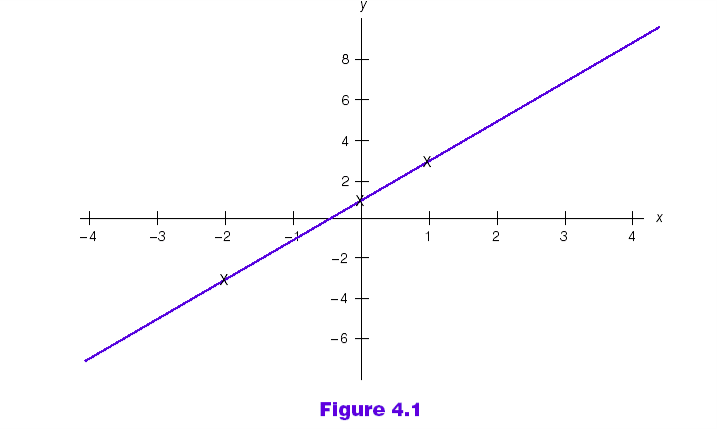
\includegraphics[scale=0.5]{F401.png} %\qquad \qquad
  \end{figure}
  $y = 2x + 1$
\end{frame}
%%%%%%%%%%%%%%%%%%%%%%%%%%%%%%%%%%%%%%%%%%%
\livelloA{$y = -3+2$}
\livelloB{Modelling Using Straight Lines}
\begin{frame}
$x$  -5   -4   -3  -2  -1   0   1   2   3     4    5

$y$ 17  14  11   8   5   2  -1  -4  -7  -10  -13


  \begin{figure}
    \centering
    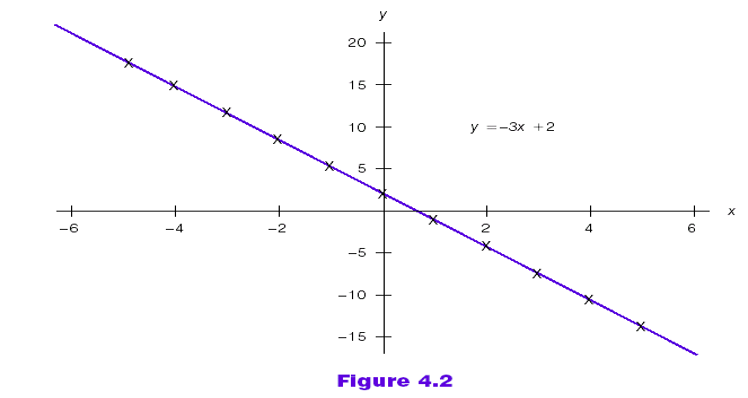
\includegraphics[scale=0.5]{F402.png} %\qquad \qquad
  \end{figure}
  $y = 2x + 1$
\end{frame}
%%%%%%%%%%%%%%%%%%%%%%%%%%%%%%%%%%%%%%%%%%%
\livelloA{Linear Equations}
\livelloB{Modelling Using Straight Lines}
\begin{frame}
\begin{itemize}
  \item y = ax + b
  \vspace*{.35mm}
  \item y = 2x + 1
  \item 3y - 3 = x
  \item 2x - 4y = 5
\end{itemize}
  \begin{figure}
    \centering
    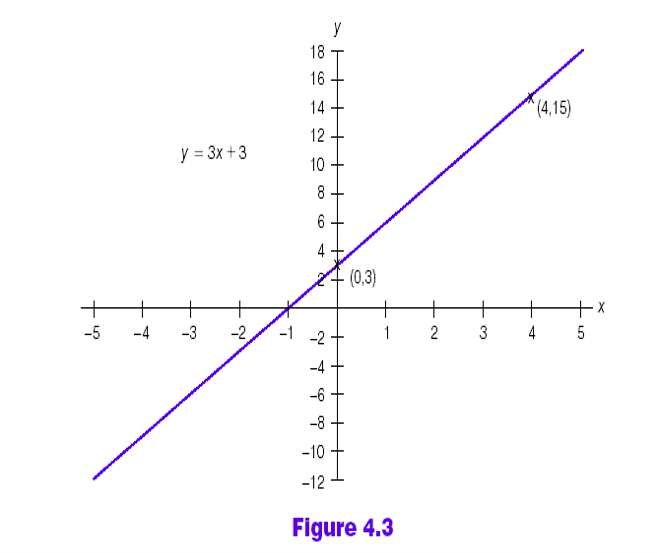
\includegraphics[scale=0.4]{F403.png} %\qquad \qquad
  \end{figure}
\end{frame}
%%%%%%%%%%%%%%%%%%%%%%%%%%%%%%%%%%%%%%%%%%%
\livelloA{Special Cases}
\livelloB{Modelling Using Straight Lines}
\begin{frame}
  \begin{figure}
    \centering
    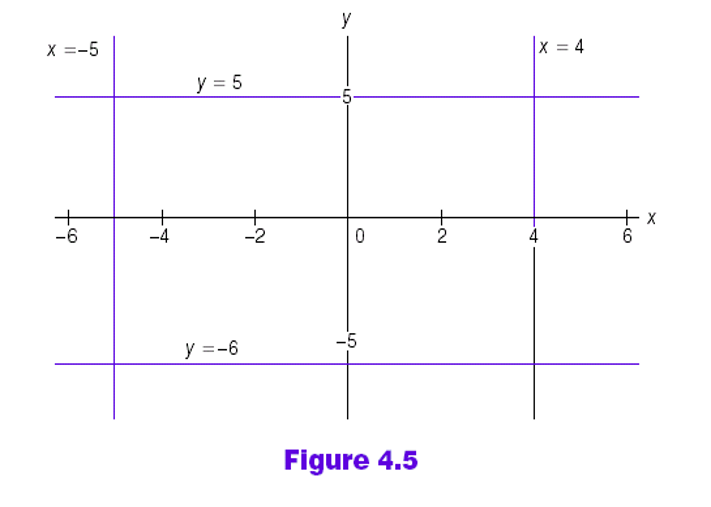
\includegraphics[scale=0.5]{F405.png} %\qquad \qquad
  \end{figure}
\end{frame}
%%%%%%%%%%%%%%%%%%%%%%%%%%%%%%%%%%%%%%%%%%%
\livelloA{b is the intercept of the y axis}
\livelloB{Modelling Using Straight Lines}
\begin{frame}
  \begin{figure}
    \centering
    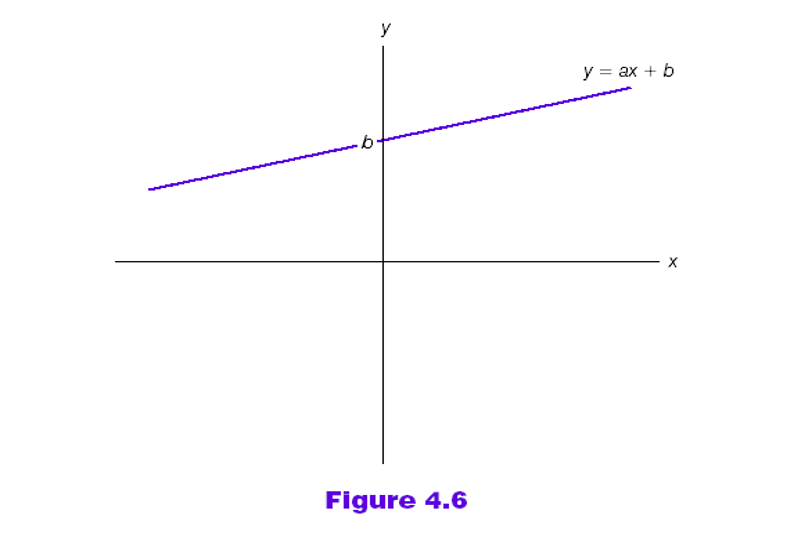
\includegraphics[scale=0.5]{F406.png} %\qquad \qquad
  \end{figure}
\end{frame}
%%%%%%%%%%%%%%%%%%%%%%%%%%%%%%%%%%%%%%%%%%%
\livelloA{a is the gradient}
\livelloB{Modelling Using Straight Lines}
\begin{frame}
  \begin{figure}
    \centering
    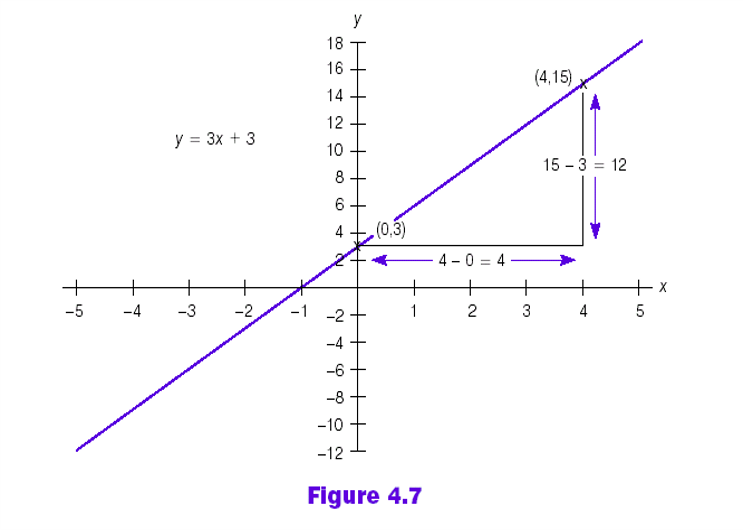
\includegraphics[scale=0.5]{F407.png} %\qquad \qquad
  \end{figure}
\end{frame}
%%%%%%%%%%%%%%%%%%%%%%%%%%%%%%%%%%%%%%%%%%%
\livelloA{Varying a and b}
\livelloB{Modelling Using Straight Lines}
\begin{frame}
  \begin{figure}
    \centering
    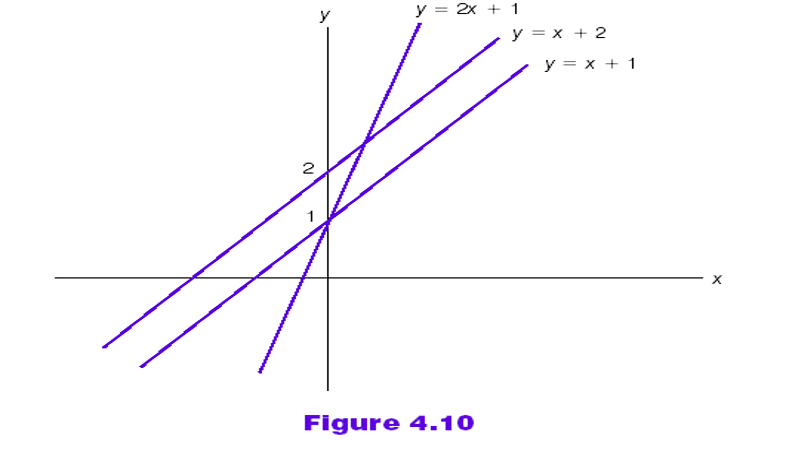
\includegraphics[scale=0.5]{F410.png} %\qquad \qquad
  \end{figure}
\end{frame}
%%%%%%%%%%%%%%%%%%%%%%%%%%%%%%%%%%%%%%%%%%%
\livelloA{Positive and negative gradients}
\livelloB{Modelling Using Straight Lines}
\begin{frame}
  \begin{figure}
    \centering
    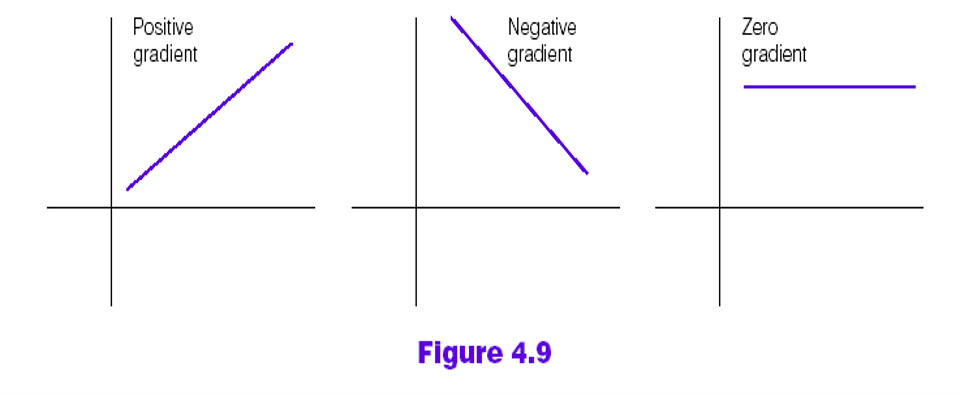
\includegraphics[scale=0.5]{F409.png} %\qquad \qquad
  \end{figure}
\end{frame}
%%%%%%%%%%%%%%%%%%%%%%%%%%%%%%%%%%%%%%%%%%%
\livelloA{Finding the equation of a line}
\livelloB{Modelling Using Straight Lines}
\begin{frame}
\begin{itemize}
   \item You only need two points to draw a straight line
   \item Find the equation of the line through the points $(-1,3)$ and $(2,9)$

   \item Gradient  is: $\frac{y2 - y1}{x2 - x1} $%= frac{9-3}{2+1} = \frac{6}{3} = 2 \Rightarrow y = 2x + b$

   \item To find the value of $b$, just use one of the points. For instance $(2,9)$ tells us that $9 = 2 x 2 + b$, so $b$ is $5$
   \item the equation is $y = 2x + 5$
\end{itemize}
\end{frame}
%%%%%%%%%%%%%%%%%%%%%%%%%%%%%%%%%%%%%%%%%%%
\livelloA{Example: budget constraint}
\livelloB{Modelling Using Straight Lines}
\begin{frame}
\begin{itemize}
   \item Company has \$2000 per week to spend making radios and televisions. It costs \$5 to make a radio, \$40 to make a television
   \item Draw a graph to show the possible numbers of radios (x) and televisions (y)  they could manufacture
\end{itemize}
 \begin{figure}
    \centering
    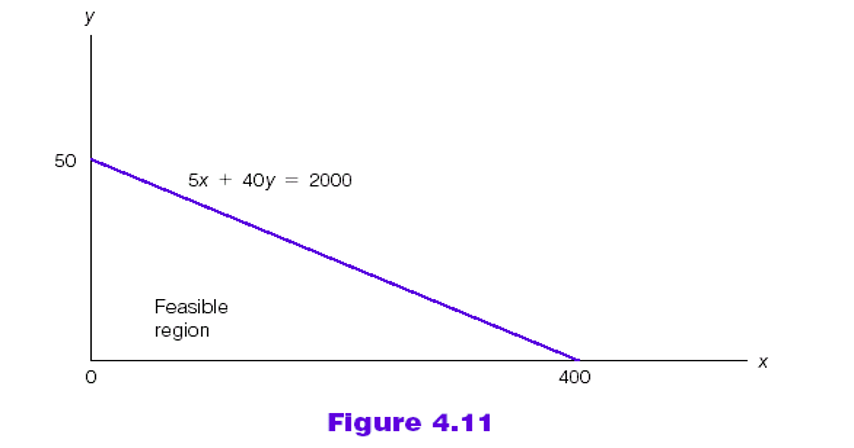
\includegraphics[scale=0.5]{F411.png} %\qquad \qquad
  \end{figure}
\end{frame}

%%%%%%%%%%%%%%%%%%%%%%%%%%%%%%%%%%%%%%%%%%%
\livelloA{Pairs of Linear Equations: supply and demand}
\livelloB{Modelling Using Straight Lines}
\begin{frame}
\begin{itemize}
   \item $Q = -\frac{1}{2}P + 100$  Demand equation
   \item $Q = 2P - 20$ Supply equation
   \item Notice negative and positive slopes
   \item Market is in equilibrium at the values of Q and P, which makes both equations true
\end{itemize}
 \begin{figure}
    \centering
    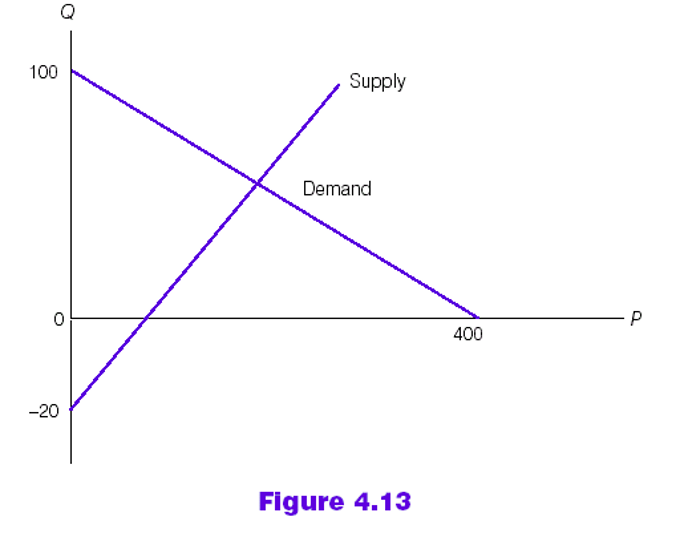
\includegraphics[scale=0.4]{F413.png} %\qquad \qquad
  \end{figure}
\end{frame}
%%%%%%%%%%%%%%%%%%%%%%%%%%%%%%%%%%%%%%%%%%%
\livelloA{Solving pairs of linear equations}
\livelloB{Modelling Using Straight Lines}
\begin{frame}
Example: we want the x and y which makes both equations true

$$ \begin{cases}
  2x - y = -1\\
  14x + 3y = 43
\end{cases} $$

Multiplying equation 1 by 3 gives

$$ \begin{cases}
  6x - 3y = -3\\
  14x + 3y = 43
\end{cases} $$

If we put x =2 into equation 1 we can solve for y

$$2x-y= -1  \Rightarrow   4-y = -1, \Rightarrow y = 5$$

Therefore: $ x = 2 ;  y = 5$

\end{frame}
%%%%%%%%%%%%%%%%%%%%%%%%%%%%%%%%%%%%%%%%%%%%%
\livelloA{Formal procedure for solving pairs of linear equations}
\livelloB{Modelling Using Straight Lines}
\begin{frame}
\begin{itemize}
   \item Multiply both sides of one equation by a number that makes the same term ( or its negative) appear in both equations
  \item Add or subtract the two equations so that these two identical terms become 0.
  \item This new equation only contains one variable so solve for this
  \item Substitute your solution for that variable into one of the original equations to solve.
\end{itemize}
\end{frame}
%%%%%%%%%%%%%%%%%%%%%%%%%%%%%%%%%%%%%%%%%%%%%
\livelloA{Sometimes there is no solution. Pparallel lines}
\livelloB{Modelling Using Straight Lines}
\begin{frame}
 \begin{figure}
    \centering
    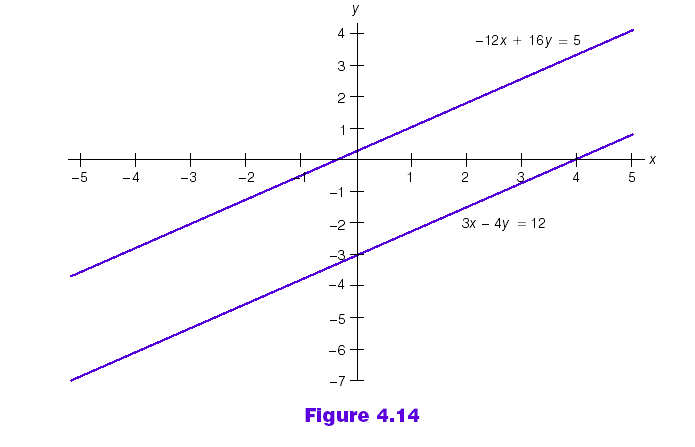
\includegraphics[scale=0.5]{F414.png} %\qquad \qquad
  \end{figure}
\end{frame}
%%%%%%%%%%%%%%%%%%%%%%%%%%%%%%%%%%%%%%%%%%%%%
\livelloA{Supply and demand example}
\livelloB{Modelling Using Straight Lines}
\begin{frame}

$$ \begin{cases}
  Q = -\frac{1}{2}P + 100 \\
  Q = 2P - 20
\end{cases} $$

Subtracting equation 1 from equation 2:
$$0 = \frac{5P}{2} -120 \Rightarrow  \frac{5P}{2} = 120  \Rightarrow P = 48$$

Substituting in equation 2:
$$Q = 96 - 20 \Rightarrow Q = 76$$

The solution is $P = 48$ and $Q = 76$

\end{frame}









\end{document}
